\section{Introdução}\label{sec}


\section{Nova sessão} % (fold)
\label{sec:nova_sess_o}

\lipsum[2]		%enchedor de linguiça em latin, apenas paragrafo 2

\onecolumn
\lstinputlisting[ %
	language=Tex, %
	caption={Exemplo de código}] %
	{./conteudo/conteudo.tex}
\onecolumn

\lipsum[3-6]		%enchedor de linguiça em latin, apenas paragrafo 4

\onecolumn
\begin{usecase}
    \addtitle{Caso de Uso 1}{Exemplo de caso de uso}

    \addfield{Resumo:}{\lipsum[1]}

    \addfield{Ator Primario:}{Manolo}

    \addfield{Pré-condições:}{Aplicativo instalado}
\end{usecase}
\onecolumn

\lipsum

\onecolumn
\begin{figure}[h]
  \begin{center}
    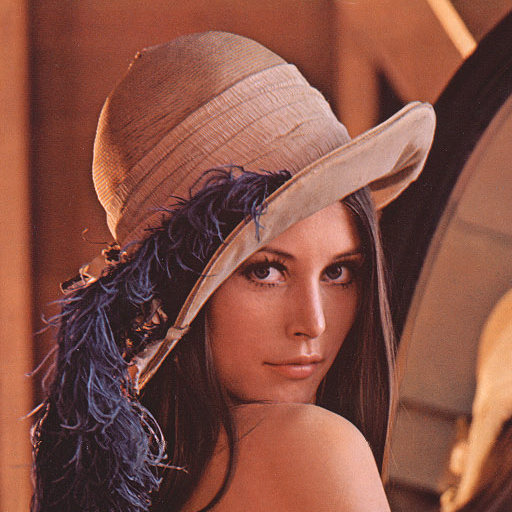
\includegraphics[width=0.8\textwidth]{conteudo/lena}
    \caption{Clássica Lena}
  \end{center}
\end{figure}
\onecolumn

\lipsum[6]
\onecolumn

\begin{longtable}{  c  L{1.5cm}  C{1.2cm}  R{2.5cm}  p{2cm}  m{3.5cm}  }
\caption{Entidade: Motorista}\\
\toprule
Nome & Tipo & Tamanho  & Restrições de Domínio & Regra de Derivação & Observações \\ \midrule
\rowcolor[gray]{0.9}
CNH & Integer & 11 & - & - & Campo que armazena o número da CNH \\
Nome & Char & 30 & - & - & Campo que armazena o nome do motorista \\
\rowcolor[gray]{0.9}
CPF & Char & 20 & Somente números & - & Campo que armazena o número do CPF \\
RG & Char & 20 & Somente números & - & Campo que armazena o número de RG \\ \bottomrule
\end{longtable}

\onecolumn

